


\selectlanguage{ngerman}%
\frenchspacing%
\begin{ledgroupsized}[r]{120mm}%
\footnotesize%
\pstart%
\noindent%
\textbf{Überlieferung:}%
\pend%
\end{ledgroupsized}%
\begin{ledgroupsized}[r]{114mm}%
\footnotesize%
\pstart%
\parindent -6mm%
\makebox[6mm][l]{\textit{L}}%
Aufzeichnung:
LH~XXXVII\;4 Bl.\;149--150.
Zwei Blatt 2\textsuperscript{o},
die ursprünglich einen Bogen gebildet haben dürften;
Wasserzeichen im Bl.\;\href{\Scan{LH_37_04_150wz}}{150};
Ränder zum Teil ausgefranst mit geringfügigem Textverlust auf Bl.\;\href{\Scan{LH_37_04_150r}}{150\,r\textsuperscript{o}} %
u.\;\href{\Scan{LH_37_04_150v}}{150\,v\textsuperscript{o}}:
Papiererhaltungsmaßnahmen.
Vier Seiten;
Textfolge nach Blattzählung (nicht von Leibniz festgelegt).
Die Schreibweise einzelner Personennamen ist uneinheitlich.
\pend%
\end{ledgroupsized}%
\selectlanguage{latin}%
\frenchspacing%
\vspace{8mm}%
\normalsize%
\pstart%
\noindent%
\lbrack%
\href{\Scan{LH_37_04_149r}}%
{149\,r\textsuperscript{o}}%
\rbrack\
\edlabel{LH_37_04_149-150_149r_ersterTeil-1}%
\edtext{%
Bernardus Ramazzinus%
\indexN{\textls{Ramazzini} (Ramazzinus), Bernardino 1633\textendash1714}
\edtext{%
medicus%
\indexS{medicus}
non minus varia doctrina%
\indexS{doctrina varia}
quam naturae scientia%
\indexS{scientia naturae}
commendabilis%
}{%
\lemma{medicus}%
\Bfootnote{%
\textit{(1)}~doctissim %
\textit{(2)}~non minus %
\lbrack...\rbrack\ scientia commendabilis%
~\textit{L}%
}}
nuper dissertationem edidit de Barometro,%
\indexS{dissertatio de barometro}%
\indexS{barometrum}
cui suas intexuit
\edtext{%
\textit{Ephemerides Barometricas}%
\indexS{ephemeris barometrica}
rationemque quaesivit%
\indexS{ratio quaesita}%
}{%
\lemma{\textit{Ephemerides}}%
\Bfootnote{%
\bars{\textit{Barometricas} \textit{erg.}} rationemque
\bars{causae \textit{gestr.}} quaesivit%
~\textit{L}%
}}
cur aere%
\indexS{aer pluvius}
\edtext{%
pluvio Hydrargyrum descendat,%
\indexS{hydrargyrum descendens}%
}{%
\lemma{pluvio}%
\Bfootnote{%
\textit{(1)}~aer d %
\textit{(2)}~Mercurius\indexS{mercurius descendens} %
\textit{(3)}~Hydrargyrum descendat,%
~\textit{L}%
}}
sereno ascendat:%
\indexS{aer serenus}%
\indexS{hydrargyrum ascendens}%
}{%
\lemma{Bernardus \lbrack...\rbrack\ ascendat}%
\Cfootnote{%
Siehe \textsc{B.\;Ramazzini},
\textit{Ephemerides barometricae Mutinenses anni m.dc.xciv, una cum disquisitione causae ascensus ac descensus mercurii in Torricelliana fistula iuxta diversum aeris statum}
(Modena 1695; Augsburg 1696).%
\cite{01516}\cite{01517}%
}}
\edtext{%
\edlabel{LH_37_04_149-150_149r_borelli-1}%
Nimirum Joh. Alphonsus Borellus%
\indexN{\textls{Borelli} (Borellus), Giovanni Alfonso 1608\textendash1679}
philosophus%
\indexS{philosophus}
et Mathematicus%
\indexS{mathematicus}
\edtext{%
egregius in libro%
\indexS{liber}
\textit{de Motionibus a gravitate pendentibus}
dicere visus est%
}{%
\lemma{egregius}%
\Bfootnote{%
\textit{(1)}~statuerat %
\textit{(2)}~dic %
\textit{(4)}~in libro \lbrack...\rbrack\ visus est%
~\textit{L}%
}}
aerem pluvium esse%
\indexS{aer pluvius}%
\indexS{aer serenus}
\edtext{%
sereno%
}{%
\lemma{sereno}%
\Bfootnote{%
\textit{erg.\;L}%
}}
graviorem,%
\indexS{aer gravior}
ob aquas scilicet admistas,%
\indexS{aqua admista aeri}
ideoque debere ab
\edtext{%
eo Hydrargyrum%
\indexS{hydrargyrum ascendens}%
}{%
\lemma{eo}%
\Bfootnote{%
\textit{(1)}~Mercur %
\textit{(2)}~Hydrargyrum%
~\textit{L}%
}}
attolli
\edtext{%
altius,
quod contra sereno coelo%
\indexS{coelum serenum}
dum aer minus obnititur%
\indexS{aer minus obnixus}
praevalente gravitate sua%
\indexS{gravitas aeris}
descendat.%
\edlabel{LH_37_04_149-150_149r_borelli-2}%
}{%
\lemma{altius,}%
\Bfootnote{%
\textit{(1)}~sereno aer %
\textit{(2)}~Idem %
\textit{(3)}~quod contra sereno caelo %
\textit{(a)}~descendat %
\textit{(aa)}~aere minus obnitente %
\textit{(bb)}~dum aer minus obnititur %
\textit{(b)}~dum aer %
\lbrack...\rbrack\ sua descendat.%
~\textit{L}%
}}%
}{%
\lemma{Nimirum \lbrack...\rbrack\ descendat}%
\Cfootnote{%
Siehe
\textsc{G.\:A.\;Borelli},
\textit{De motionibus naturalibus a gravitate pendentibus},
prop.\;113 u.\;115
(Bologna 1670, S.\;239\,f. u.\;242).%
\cite{02068}
Leibnizens unmittelbare Quelle ist wohl aber \textsc{Ramazzini}, \textit{Ephemerides barometricae} (1695, S.\;2\,f.; 1696, S.\;1), wie seine Wendung \textit{dicere visus est} nahelegt.%
\cite{01516}\cite{01517}%
}}
Cum vero cl.
\edtext{%
\edtext{%
Ramazzinus%
\indexN{\textls{Ramazzini} (Ramazzinus), Bernardino 1633\textendash1714}
Barometricas observationes%
\indexS{observatio barometrica}%
}{%
\lemma{Ramazzinus}%
\Bfootnote{%
\textit{(1)}~experi %
\textit{(2)}~Barometricas observationes%
~\textit{L}%
}}
non ita dudum instituisset
\edtext{%
integroque anno continuasset,%
}{%
\lemma{integroque anno continuasset}%
\Bfootnote{%
\textit{erg.\;L}%
}}
contrarium prorsus accidere miratus%
}{%
\lemma{Ramazzinus \bracks{...} miratus est}%
\Cfootnote{%
Vgl. a.a.O. %
(1695, S.\;2;\cite{01516} 1696, S.\;1).\cite{01517}%
}}
\edtext{%
est.
Nempe sereno coelo%
\indexS{coelum serenum}
ascendere Mercurium,%
\indexS{mercurius ascendens}
quasi aere facto graviore,%
\indexS{aer gravior}
\ledpb%
contra pluvia tempestate%
\indexS{tempestas pluvia}
subsidere.%
\indexS{mercurius subsidens}
\edtext{%
Idem postea ab aliis observatum
notavit.%
}{%
\lemma{Idem \bracks{...} notavit}%
\Cfootnote{%
Vgl. a.a.O. %
(1695, S.\;4--7;\cite{01516} 1696, S.\;2\,f.).\cite{01517}
Erwähnt werden dort u.\,a. die Beobachtungen von 
J.\;d'Alencé,\indexN{\textls{Alencé} (d'Alancé, Dalancé, Dalancay, Dalencé), Joachim de 1640\textendash1707}
C.\;Comiers\indexN{\textls{Comiers}, Claude, gest. 1693}
und O.\;v.\:Guericke.\indexN{\textls{Guericke} (Gerickius, Gericke), Otto von 1602\textendash1686}%
}}%
}{%
\lemma{est.}%
\Bfootnote{%
\textit{(1)}~Idemque mox aliis %
\textit{(2)}~Nempe sereno %
\lbrack...\rbrack\ facto graviore, %
\textit{(a)}~leviore, %
\textit{(b)}~contra pluvia %
\lbrack...\rbrack\ postea ab %
\textit{(aa)}~aliis %
\textit{(bb)}~\bars{ab \textit{streicht Hrsg.}} aliis observatum notavit.%
~\textit{L}%
}}
\edtext{%
\edlabel{LH_37_04_149-150_149r_fee-1}%
Causas igitur paradoxi%
\indexS{causa paradoxi}%
\indexS{paradoxon}%
\indexS{causa inquisita}
inquirere %
peculiari dissertatione%
\indexS{dissertatio peculiaris}
instituit;
et aliorum doctissimorum virorum%
\indexS{vir doctus}
sententias
\edlabel{37_04_149-150_01a}%
adjecit.%
\indexS{sententia virorum doctissimorum}%
\edlabel{LH_37_04_149-150_149r_fee-2}%
}{%
\lemma{Causas \lbrack...\rbrack\ adjecit}%
\Cfootnote{%
Vgl. a.a.O. %
(1695, S.\;31\,f.;\cite{01516} 1696, ab S.\;12).\cite{01517}
Siehe zudem die Erläuterung zu N.\ref{53442}, \refpassage{LH_37_04_151_151r_anspiel-3}{LH_37_04_151_151r_anspiel-2} im vorliegenden Band.%
}}%
\edtext{}{%
\xxref{37_04_149-150_01a}{37_04_149-150_01b}%
\lemma{adjecit.}%
\Bfootnote{%
\textit{(1)}~Equidem verissimum est %
\textit{(2)}~Est autem res utique inquisitu digna, %
\textit{(a)}~quam primus quod %
\textit{(b)}~sin et %
\textit{(3)}~Ottono Gerikio\indexN{\textls{Guericke} (Gerickius, Gericke), Otto von 1602\textendash1686} %
\bars{consule Magdeburgensi~\textit{erg.}}, primo Antliae pneumaticae\indexS{antlia pneumatica} a Rob. Boilio\indexN{\textls{Boyle} (Boylius, Boyl), Robert 1627\textendash1691} %
\textit{(4)}~Bar %
\textit{(5)}~Est autem \lbrack...\rbrack\ dignissima primus %
\textit{(a)}~Torricellius\indexN{\textls{Torricelli} (Torricellius), Evangelista 1608\textendash1647} invenit %
\textit{(b)}~Galilaeus\indexN{\textls{Galilei} (Galilaeus, Galileus), Galileo 1564\textendash1642} rem a mechanicis compertam prodidit, %
\textit{(aa)}~aere %
\textit{(bb)}~non %
\textit{(cc)}~antlias aspirantes, %
\lbrack...\rbrack\ pedes attollere.%
~\textit{L}%
}}
\pend%
\pstart%
Est autem tota res inquisitione accuratiore dignissima%
\indexS{inquisitio accuratior}%
\indexS{res digna inquisitione}%
\lbrack:\rbrack\
primus
\edtext{%
Galilaeus%
\indexN{\textls{Galilei} (Galilaeus, Galileus), Galileo 1564\textendash1642}
rem a mechanicis compertam%
\indexS{res comperta a mechanicis}\indexS{mechanicus}
prodidit,
antlias aspirantes,%
\indexS{antlia aspirans}
quas vocant%
\lbrack,\rbrack\
aquam non nisi ad 30 circiter pedes attollere.%
\indexS{aqua elevata ad 30 pedes}%
\indexS{pes}%
\edlabel{37_04_149-150_01b}%
}{%
\lemma{Galilaeus \lbrack...\rbrack\ attollere}%
\Cfootnote{%
Siehe G.\;\textsc{Galilei},
\textit{Discorsi}, giornata I
(Leiden 1638, S.\;17;\cite{00050}
\textit{GO}~VIII, S.\;63\,f.).\cite{00048}
Dort ist von \textit{diciotto braccia} die Rede.%
}}
\edtext{%
Torricellius%
\indexN{\textls{Torricelli} (Torricellius), Evangelista 1608\textendash1647}
deprehendit similiter
Hydrargyrum non posse attolli%
\indexS{hydrargyrum eductum in altum}
\edtext{%
nisi%
}{%
\lemma{nisi}%
\Bfootnote{%
\textit{erg.\;L}%
}}
ad altitudinem%
\indexS{altitudo hydrargyri in barometro}
quae hujus sit pars circiter decima quarta,
quia tanto gravior est Mercurius aqua.%
\indexS{mercurius gravior aqua}
Unde videns rem pendere ab aequilibrio liquorum%
\indexS{aequilibrium liquorum}%
\indexS{liquor in aequilibrio}
\edtext{%
invenit oppositum columnae aereae%
}{%
\lemma{invenit}%
\Bfootnote{%
\textit{(1)}~aeris oppo %
\textit{(2)}~oppositum columnae aereae%
~\textit{L}%
}}
pondus%
\indexS{pondus columnae aereae}%
\indexS{columna aerea}
veram esse huius aquae vel
\edtext{%
Hydrargyri in altum eductionis causam,%
\indexS{causa eductionis aquae in altum}%
\indexS{causa eductionis hydrargyri in altum}%
\indexS{eductio aquae in altum}%
\indexS{eductio hydrargyri in altum}%
\indexS{aqua educta in altum}%
\indexS{hydrargyrum eductum in altum}
et comperit%
}{%
\lemma{Hydrargyri}%
\Bfootnote{%
\textit{(1)}~suspensionis causam, et deprehend\indexS{causa suspensionis hydrargyri}\indexS{suspensio hydrargyri in tubo Torricelliano} %
\textit{(2)}~in altum eductionis, et comperit%
~\textit{L}%
}}
Mercurium ad 27 pollices circiter suspensum%
\indexS{mercurius suspensus ad 27 pollices}%
\indexS{suspensio mercurii in tubo Torricelliano}%
\indexS{pollex}
manere in
\edtext{%
Tubo verticaliter erecto%
\indexS{tubus Torricellianus}
supra clauso,
infra aperto.%
}{%
\lemma{Tubo}%
\Bfootnote{%
\textit{(1)}~infra %
\textit{(2)}~supra %
\textit{(3)}~claus %
\textit{(4)}~perpendicu %
\textit{(5)}~verticaliter erecto %
\lbrack...\rbrack\ infra aperto.%
~\textit{L}%
}}%
}{%
\lemma{Torricellius \lbrack...\rbrack\ aperto}%
\Cfootnote{%
Siehe zum Experiment mit dem Quecksilber
E.\;\textsc{Torricelli}, %
Brief an M.\;Ricci vom 11.\;Juni 1644%
\cite{00107}
(C.\;\textsc{Dati},
\textit{Lettera a Filaleti}, %
Florenz 1663, S.\;20\,f.;%
\cite{00032}
\textit{TO} III, S.\;186--188).\cite{00108}%
}}
Postea experimentum%
\indexS{experimentum Torricellianum prosecutum}
prosecuti sunt
\edtext{%
Blasius Pascalius%
\indexN{\textls{Pascal} (Pascalius), Blaise 1623\textendash1662}
in Gallia,%
\indexO{Frankreich}
vir celebris%
\indexS{vir celebris}
qui primus
\edtext{%
notavit Mercurium%
}{%
\lemma{notavit}%
\Bfootnote{%
\textit{(1)}~aqua %
\textit{(2)}~Mercurium%
~\textit{L}%
}}
in monte excelso subsidere,%
\indexS{mercurius subsidens in monte}%
}{%
\lemma{Blasius \lbrack...\rbrack\ subsidere}%
\Cfootnote{%
Siehe zum Experiment am Puy de Dôme\indexO{Puy de Dôme}
B.\;\textsc{Pascal},
\textit{Récit de la grande expérience}, 1648\cite{02577} %
(\textit{Traitez}, Paris 1663, S.\;165--194;\cite{00081}
\textit{PO}\;II, S.\;653--690).\cite{01524}
}}
et
\edtext{%
Otto Gerickius%
\indexN{\textls{Guericke} (Gerickius, Gericke), Otto von 1602\textendash1686}
consul%
\indexS{consul}
\edtext{%
Magdeburgicus%
\indexO{Magdeburg}
\lbrack qui\rbrack\
rem omnem maxime promovit%
\lbrack:\rbrack\
idemque mirifice%
}{%
\lemma{Magdeburgicus}%
\Bfootnote{%
\textit{(1)}~qui %
\textit{(2)}~\bars{qui \textit{erg. Hrsg.}} rem omnem %
\textit{(a)}~longius %
\textit{(b)}~maxime promovit idemque%
~\textit{L}%
}}
sibi obstrinxit harum scientiarum cultores%
\indexS{cultor scientiarum}
excogitata Antlia,%
\indexS{antlia Magdeburgica}
\ledpb%
qua aerem ex vase eduxit,%
\indexS{antlia educens aerem e vase}%
\indexS{aer eductus e vase}
infinitisque pulcherrimis experimentis%
\indexS{experimentum pulchrum}%
\indexS{experimentum demonstrans effectum aeris}
(partim ab ipsomet sumtis)
occasionem
\edtext{%
dedit%
\lbrack,\rbrack\
quibus%
}{%
\lemma{dedit}%
\Bfootnote{%
\textit{(1)}~quam %
\textit{(2)}~quibus%
~\textit{L}%
}}
usus aeris effecutsque maximi ad oculum demonstrantur.%
\indexS{effectus aeris demonstratus ad oculum}%
\indexS{oculus}%
}{%
\lemma{Otto \lbrack...\rbrack\ demonstrantur}%
\Cfootnote{%
Siehe
O.\:v.\:\textsc{Guericke},
\textit{Experimenta nova}, lib.\;III
(Amsterdam 1672, S.\;71--124).%
\cite{00055}
Dort werden die Versuche und entsprechenden Vorrichtungen beschrieben, auf die Leibniz hinweist.
Diese waren aber bereits Jahre zuvor bekannt gemacht worden;
siehe für die frühere Überlieferung etwa
C.\;\textsc{Schott},
\textit{Mechanica hydraulico-pneumatica},
Anhang: \textit{Experimentum novum Magdeburgicum}
(Frankfurt a.\,M. 1657, S.\;441--488).\cite{00095}%
}}
Quae deinde a
\edtext{%
Roberto%
\indexN{\textls{Boyle} (Boylius, Boyl), Robert 1627\textendash1691}
Boylio Armigero%
\indexS{armigerus}
\edtext{%
Anglo porro praeclare sunt exculta,
integris%
}{%
\lemma{Anglo}%
\Bfootnote{%
\textit{(1)}~egregie %
\textit{(2)}~porro praeclare sunt exculta, %
\textit{(a)}~porro idem %
\textit{(b)}~integris%
~\textit{L}%
}}
de Antlia illa Magdeburgica vel Gerickio%
\indexN{\textls{Guericke} (Gerickius, Gericke), Otto von 1602\textendash1686}%
-Boyliana%
\indexN{\textls{Boyle} (Boylius, Boyl), Robert 1627\textendash1691}%
\indexS{antlia Magdeburgica}%
\indexS{antlia Gerickio-Boyliana}
libris conscriptis.%
\indexS{liber conscriptus}%
}{%
\lemma{Roberto \lbrack...\rbrack\ conscriptis}%
\Cfootnote{%
Seine Versuche mit der Vakuumpumpe über Gewicht und Elastizität der Luft schildert R.\;\textsc{Boyle} hauptsächlich in
\textit{New experiments physico-mechanicall}
(Oxford 1660;\cite{00015}
\textit{BW}~I, S.\;141--301)\cite{00017}
und
\textit{A continuation of new experiments} %
(Oxford 1669;\cite{01062}
\textit{BW}~VI, S.\;27--187).\cite{00017}
}}%
\pend%
\pstart%
\edtext{%
Porro
Gerikius mature%
\indexN{\textls{Guericke} (Gerickius, Gericke), Otto von 1602\textendash1686}
observatis aeris variationibus%
\indexS{variationes aeris collatae cum tubo hydrargyri}
et cum Tubo Hydrargyri collatis%
\indexS{tubus hydrargyri}
indicem tempestatum praenuncium%
\indexS{index praenuncius tempestatum}
sub homunculi figura%
\indexS{figura homunculi}%
\indexS{homunculus index tempestatum}
eleganter est commentus;%
}{%
\lemma{Porro}%
\Bfootnote{%
\textit{(1)}~idem %
\textit{(2)}~Gerikius\indexN{\textls{Guericke} (Gerickius, Gericke), Otto von 1602\textendash1686} %
\textit{(a)}~primus mo %
\textit{(b)}~mature observatis aeris variationibus %
\bars{et cum Tubo Hydrargyri collatis \textit{erg.}}
indicem tempestatum %
\lbrack...\rbrack\ homunculi figura %
\textit{(aa)}~egregie %
\textit{(bb)}~eleganter est commentus;%
~\textit{L}%
}%
\lemma{Gerikius \lbrack...\rbrack\ commentus}%
\Cfootnote{%
Siehe \textsc{Guericke}, \textit{Experimenta nova},\cite{00055}
lib.\;III, cap.\;20 u.\;31 (S.\;100a--b u.\;115a--b);
lib.\;V, appendix (S.\;188b--189a).
Leibniz hatte 1672 diese Stellen exzerpiert:
Vgl. \textit{LSB} VIII,\;1 N.\;36,\cite{01197}
S.\;257.23--30; 259.1--10; 270.14--19.%
}%
}
deinde et%
\edlabel{LH_37_04_149-150_149r_rvb-1}%
\edtext{%
Hugenius%
\indexN{\textls{Huygens} (Hugenius, Ugenius, Hugens, Huguens), Christiaan 1629\textendash1695}%
}{%
\lemma{Hugenius}
\Cfootnote{%
Siehe
C.\;\textsc{Huygens},
\glqq Extrait d'une autre lettre touchant une nouvelle maniere de Barometre\grqq\
(\textit{JS}, 12.\;Dezember 1672, S.\;152--156;%
\cite{01522}
\textit{HO}~VII, S.\;238--241).%
\cite{00113}%
}}
et%
\edtext{%
Hookius%
\indexN{\textls{Hooke} (Hookius, Hook), Robert 1635\textendash1703}%
}{%
\lemma{Hookius}
\Cfootnote{%
Siehe
\textsc{R.\;Hooke},
\textit{Micrographia}, Preface
(London 1665, S.\:[c3] u.\;Tafel I, Abb.\;I);%
\cite{00061}
\textsc{Ders.},
\glqq A new Contrivance of Wheel-Barometer\grqq\
(\textit{PT}, 4.\;Juni 1666,
S.\;218\,f. u.\;Abb.\;1 vor S.\;215).%
\cite{01523}%
}}
\edtext{%
aliique%
}{%
\lemma{aliique}%
\Bfootnote{%
~\textit{erg.\;L}%
}}
alias machinationes elegantes excogitavere,%
\indexS{machinatio elegans excogitata}
\edtext{%
quibus instrumentum%
}{%
\lemma{quibus}%
\Bfootnote{%
\textit{(1)}~Barometrum\indexS{barometrum} %
\textit{(2)}~instrumentum%
~\textit{L}%
}}
redditum est multo aptius ad aeris variationes%
\indexS{instrumentum ad variationes aeris indicandas}%
\indexS{variationes aeris minimae} 
\edtext{%
minimas indicandas,%
\edlabel{LH_37_04_149-150_149r_rvb-2}%
}{%
\lemma{minimas}%
\Bfootnote{%
\textit{(1)}~observandas %
\textit{(2)}~iudicandas%
~\textit{L}%
}}
unde tandem
\lbrack%
\href{\Scan{LH_37_04_149v}}%
{149\,v\textsuperscript{o}}%
\rbrack\
communi consensu%
\indexS{consensus communis}
Barometri%
\indexS{barometrum}
appellatio%
\indexS{appellatio barometri}
invaluit,
quia hoc Tubo aeris gravitatem metiri%
\indexS{gravitas aeris}%
\indexS{mensuratio gravitatis aeris}
\edtext{%
licet.
Fuere viri docti%
\indexS{vir doctus}%
}{%
\lemma{licet.}%
\Bfootnote{%
\textit{(1)}~Et %
\textit{(2)}~Extant autem complures Barometricae observationes apud\indexS{observatio barometrica} %
\textit{(a)}~Gerick\indexN{\textls{Guericke} (Gerickius, Gericke), Otto von 1602\textendash1686} %
\textit{(b)}~Pascalium,\indexN{\textls{Pascal} (Pascalius), Blaise 1623\textendash1662} Gerikium, Boylium\indexN{\textls{Boyle} (Boylius, Boyl), Robert 1627\textendash1691} %
\textit{(3)}~Fuere viri docti%
~\textit{L}%
}}
qui instrumentum hoc%
\indexS{instrumentum ad variationes aeris indicandas}
\edtext{%
cum Thermometro%
\indexS{thermometrum}
et Hygrometro%
\indexS{hygrometrum}
conju\lbrack n\rbrack xere;%
\indexS{barometrum conjunctum cum hygrometro et thermometro}%
}{%
\lemma{cum}%
\Bfootnote{%
\textit{(1)}~Barometro et %
\textit{(2)}~Thermometro et Hygrometro %
\textit{(a)}~comp %
\textit{(b)}~conjugerunt %
\textit{(c)}~\bars{conjuxere%
~\textit{ändert Hrsg.}}%
\textit{L}%
}}
inque ea re non exiguum posuit studium%
\indexS{studium}
v.\;cl.\;Sam.\;Reiherus,%
\indexN{\textls{Reyher} (Reiherus, Reiher), Samuel 1635\textendash1714}%
\indexS{vir clarus}
Jureconsultus%
\indexS{jureconsultus}
et
\edtext{%
Mathematicus%
\indexS{mathematicus}
chiloniensis%
\indexO{Kiel}
doctissimus, %
}{%
\lemma{Mathematicus}%
\Bfootnote{%
\textit{(1)}~et %
\textit{(2)}~chiloniensis %
\textit{(a)}~egregius %
\textit{(b)}~doctissimus,%
~\textit{L}%
}}%
\edtext{%
qui tabulas aliquas suas%
\indexS{tabulae Reiheri}
et observationes%
\indexS{observationes Reiheri}
ante complures annos mihi communicavit.%
}{%
\lemma{qui \lbrack...\rbrack\ communicavit}%
\Cfootnote{%
Siehe die Beilage zu
S.\;\textsc{Reyher}, Brief an G.\,W.\;Leibniz vom 24.\;August (3.\;September) 1679
(\textit{LSB} III,\;2 N.\;339).\cite{01518}\cite{01434}%
}}
Nec dubitem
collata opera%
\indexS{opera collata}
multa hic quoque erui posse
magni non ad rem tantum nauticam%
\indexS{res nautica}
et agricultoriam%
\indexS{res agricultoria}
sed et medicam%
\indexS{res medica}
ipsam momenti futura.
Certe
\edtext{%
Gerikius%
\indexN{\textls{Guericke} (Gerickius, Gericke), Otto von 1602\textendash1686}
observavit
\ledpb%
magnas tempestates%
\indexS{tempestas praesagita}
insolita Mercurii subsidentia%
\indexS{subsidentia mercurii insolita}%
\indexS{mercurius subsidens}
praesagiri.
\edtext{%
Itaque prodesse navigantibus posset Barometrum,%
\indexS{barometrum magno usui navigantibus}
ut%
}{%
\lemma{Itaque}%
\Bfootnote{%
\textit{(1)}~si naut %
\textit{(2)}~magnus %
\textit{(3)}~magno usui navigantibus esse posset %
\textit{(4)}~prodesse navigantibus posset Barometrum %
\textit{(a)}~ad %
\textit{(b)}~ut%
~\textit{L}%
}}
vel mature in portum%
\indexS{navigans receptus in portum}%
\indexS{portus}
se recipiant,
vel certe
\edlabel{37_04_149-150_149v_02a}%
a brevibus scopulisque recedant.%
\indexS{navigans recedens a brevibus scopulisque}%
\indexS{brevia}%
\indexS{scopulus}%
\edtext{}{%
\xxref{37_04_149-150_149v_02a}{37_04_149-150_149v_02b}
\lemma{a}%
\Bfootnote{%
\textit{(1)}~locis recede %
\textit{(2)}~brevibus scopulisque recedant %
\textit{(a)}~Sed %
\textit{(b)}~Caeterum%
~\textit{L}%
}}%
}{%
\lemma{Gerikius \lbrack...\rbrack\ recedant}%
\Cfootnote{%
Siehe \textsc{Guericke}, \textit{Experimenta nova},%
\cite{00055}
lib.\;V, appendix (S.\;195b--196a).
Leibniz hatte 1672 diese Stelle exzerpiert;
vgl. \textit{LSB} VIII,\;1 N.\;36,%
\cite{01197}
S.\;270.21--25.}}
\pend%
\pstart%
\edlabel{37_04_149-150_149v_causa-1}%
Caeterum%
\edlabel{37_04_149-150_149v_02b}
quod causam paradoxi%
\indexS{causa paradoxi}%
\indexS{paradoxon}
attinet%
\lbrack,\rbrack\
equidem verisimillimum mihi semper visum
\edtext{%
est aerem pluvium%
\indexS{aer pluvius}
et pluviam minantem%
\indexS{aer minans pluviam}%
\indexS{pluvia}
esse leviorem,%
\indexS{aer levior}
quia cadentes jam guttas%
\indexS{gutta pluvia}%
\indexS{gutta sustenta ab aere}
non amplius sustinet%
\indexS{aer sustinens guttas}
exoneratusque%
\indexS{aer exoneratus}
adeo partem ponderis sui amittit;%
\indexS{pondus aeris}
contra serena tempestate%
\indexS{tempestas serena}%
}{%
\lemma{est}%
\Bfootnote{%
\textit{(1)}~aere pluvio %
\textit{(2)}~aerem pluvium %
\textit{(a)}~aut paulo %
\textit{(b)}~et ante %
\textit{(c)}~et %
\textit{(d)}~allevari\lbrack\textit{!}\rbrack\ %
\textit{(e)}~et %
\textit{(f)}~velut exonerari %
\textit{(g)}~et pluviam %
\lbrack...\rbrack\ leviorem, quia %
\textit{(aa)}~a %
\textit{(bb)}~cadentes jam %
\lbrack...\rbrack\ amplius sustinet %
\textit{(aaa)}~; contra aer %
\textit{(bbb)}~exoneratusque adeo %
\lbrack...\rbrack\ amittit; contra %
\textit{(aaaa)}~aere sereno %
\textit{(bbbb)}~serena %
\mbox{\bars{tempestate \textit{erg.}}%
\textit{L}}%
}}
aquam attenuatam%
\indexS{aqua attenuata sustenta ab aere}
et dispersam%
\indexS{aqua dispersa sustenta ab aere}
ab aere%
\indexS{aer sustinens aquam attenuatam et dispersam}
susteneri
ac proinde %
cum ipso in subjectum Mercurium%
\indexS{mercurius subjectus gravitati aeris}
\edtext{%
gravita\lbrack r\rbrack e.%
}{%
\lemma{gravitate}%
\Bfootnote{%
\textit{L\;ändert Hrsg.}%
}}%
\edlabel{37_04_149-150_149v_causa-2}
\edtext{%
Eamque sententiam%
\indexS{sententia innuta}
\edtext{%
dudum innuere%
}{%
\lemma{dudum}%
\Bfootnote{%
\textit{(1)}~indicare %
\textit{(2)}~innuere%
~\textit{L}%
}}%
videntur viri docti%
\indexS{vir doctus}
quorum nonnulli etiam a cl.\;%
\edtext{%
Ramazzino%
\indexN{\textls{Ramazzini} (Ramazzinus), Bernardino 1633\textendash1714}
allegantur.%
\edlabel{LH_37_04_149-150_149r_ersterTeil-2}%
}{%
\lemma{Ramazzino}%
\Bfootnote{%
\textit{(1)}~indicantur %
\textit{(2)}~allegantur.%
~\textit{L}%
}}%
}{%
\lemma{Eamque \lbrack...\rbrack\ allegantur}%
\Cfootnote{%
Unter den in \textsc{Ramazzini}, \textit{Ephemerides barometricae} dargelegten Erklärungsvorschlägen sind vornehmlich zwei (1695, S.\;31\,f., 38;\cite{01516} 1696, S.\;12\,f.,\;15)\cite{01517} mit Leibnizens Ansatz verwandt:
der eines "autor anonymus"\indexN{\textls{Alencé} (d'Alancé, Dalancé, Dalancay, Dalencé), Joachim de 1640\textendash1707} (\textsc{J.\;d'Alencé}, \textit{Traittez des baromètres}, Amsterdam 1688,\cite{01525} S.\;45\,f.)
und derjenige von C.\;Comiers\indexN{\textls{Comiers}, Claude, gest. 1693} (bei \textsc{P.\;Le Lorrain de Vallemont}, \textit{Physique occulte}, cap.\;XI, Paris 1693,\cite{01513} Bd.\;II, S.\;355).\indexN{\textls{Le Lorrain de Vallemont} (Vallemontius), Pierre 1649\textendash1721}
}}
Sed quia rem non satis%
\indexS{res explicata distincte}
\edtext{%
distincte explicuere,
putavi sic omne clarius proponi posse.%
}{%
\lemma{distincte}%
\Bfootnote{%
\textit{(1)}~exposuere hinc %
\textit{(a)}~visum est %
\textit{(b)}~digna visa est %
\textit{(2)}~explicuere, putavi %
\lbrack...\rbrack\ proponi posse.%
~\textit{L}%
}}
\pend%
\begin{edfigure}[2.00em][0.00em]%
\includegraphics[width=0.56\textwidth]%
{gesamttex/edit_VIII-4/images/LH_37_04_149-150_d1_149v.pdf}
\edcaption[-0.50em]{\lbrack \textit{Fig.\:1}\rbrack}%
\end{edfigure}%
\newpage%
\pstart%
\edlabel{LH_37_04_149-150_149v-annahme-1}%
In
\edtext{%
libra parium brachiorum%
\indexS{libra parium brachiorum}%
\indexS{brachium librae}%
}{%
\lemma{libra parium brachiorum}%
\Cfootnote{%
Vgl. das Diagramm \lbrack\textit{Fig.\:1}\rbrack.%
}}
\textit{AB}, \textit{AC}
sint aequilibrata%
\indexS{pondus aequilibratum}%
\indexS{aequilibrium in libra}
pondus \textit{D} %
et vas \textit{E} %
aquam continens,%
\indexS{vas continens aquam}%
\indexS{aqua contena in vase}
quod sit altum potius sive profundum
quam largum.
Et in aqua natet%
\indexS{vasculum natans}
vasculum~\textit{F} ex
\edtext{%
plumbo%
\indexS{vasculum plumbeum}%
\indexS{plumbum}
vel ferro%
\indexS{vasculum ferreum}%
\indexS{ferrum}
vitrone%
\indexS{vasculum vitreum}%
\indexS{vitrum}
vel alia materia factum
quae%
}{%
\lemma{plumbo}%
\Bfootnote{%
\bars{vel \textit{erg.}} ferro vitro%
\bars{ne \textit{erg.}} vel alia materia %
\bars{factum \textit{erg.}} quae%
~\textit{L}%
}}
in aqua per se mergitur,%
\indexS{materia mergens in aqua}
hic autem ob vacuam cavitatem%
\indexS{cavitas vacua}
sustinetur.%
\indexS{materia sustenta cavitate vacua}
Sit porro in vasculo \textit{F}
foramen%
\indexS{foramen vasculi obturatum}
obturatum %
charta%
\indexS{charta obturans foramen} %
vel alia materia%
\indexS{materia obturans foramen}%
\indexS{materia perrupta ab aqua}
quam aqua paulatim perrumpat%
\indexS{aqua perrumpens chartam}%
\indexS{charta perrupta ab aqua}
et vasculum impleat;%
\indexS{aqua implens vasculum}
vasculum impletum descendet%
\indexS{vasculum impletum aqua}
et durante descensu%
\indexS{descensus vasculi in aqua}%
\indexS{vasculum descendens in aqua}%
\lbrack,\rbrack\
\edtext{%
mutato
quod erat ante descensum
aequilibrio,%
\indexS{aequilibrium mutatum}%
}{%
\lemma{mutato}%
\Bfootnote{%
\textit{(1)}~aequilibrio, %
\textit{(2)}~quod erat ante descensum aequilibrio,%
~\textit{L}%
}}
vincet pondus \textit{D} %
\edtext{%
et elevabit vas \textit{E},%
}{%
\lemma{et}%
\Bfootnote{%
\textit{(1)}~vas \textlangle \textit{E}\textrangle\ %
\textit{(2)}~elevabit vas \textit{E},%
~\textit{L}%
}}
quia a vase \textit{E} %
non amplius sustinetur vasculum \textit{F},
quippe descendens;
atque adeo vas \textit{E} de pondere suo aliquid amisit.%
\indexS{pondus amissum}
Nec vero restituetur aequilibrium,%
\indexS{aequilibrium restitutum}
\edtext{%
donec vasculum \textit{F}
ad fundum vasis \textit{E}%
}{%
\lemma{donec}%
\Bfootnote{%
\textit{(1)}~vas %
\textit{(2)}~vasculum \textit{F} %
\textit{(a)}~ad v %
\textit{(b)}~ad fundum vasis \textit{E}%
~\textit{L}%
}}
pervenerit %
ibique quieverit,
ubi scilicet rursus ab eo sustinetur.%
\edlabel{LH_37_04_149-150_149v-annahme-2}
\lbrack%
\href{\Scan{LH_37_04_150r}}%
{150\,r\textsuperscript{o}}%
\rbrack%
\pend%
\pstart%
Similiter ergo,
si
\edtext{%
cylinder aeris%
\indexS{cylinder aeris}
\textit{GH}%
}{%
\lemma{cylinder}%
\Bfootnote{%
\textit{(1)}~vasis %
\textit{(2)}~aeris \textit{GH}%
~\textit{L}%
}%
\lemma{cylinder aeris \textit{GH}}%
\Cfootnote{%
Vgl. das Diagramm \lbrack\textit{Fig.\:2}\rbrack.%
}%
}
et Hydrargyri \textit{LM}%
\indexS{hydrargyrum}
sint in aequilibrio,%
\indexS{aequilibrium aeris et hydrargyri}
erit Hydrargyrum instar ponderis \textit{D} %
et columna aeris,%
\indexS{columna aeris}
respectu
\edtext{%
aquae sustentatae%
\indexS{aqua sustentata ab aere}%
\lbrack,\rbrack\
instar%
}{%
\lemma{aquae}%
\Bfootnote{%
\textit{(1)}~inclusae instar %
\textit{(2)}~sustentatae instar%
~\textit{L}%
}}
vasis \textit{E}.
Cadente autem aqua%
\indexS{aqua cadens in aere}
cessanteque sustentatione
praevalebit Mercurius
atque adeo subsidet%
\indexS{mercurius subsidens in barometro}
\edtext{%
quemadmodum observationibus%
\indexS{observatio barometrica}%
}{%
\lemma{quemadmodum}%
\Bfootnote{%
\textit{(1)}~et %
\textit{(a)}~experientia\indexS{experientia} %
\textit{(b)}~per experientiam %
\textit{(2)}~observationibus%
~\textit{L}%
}}
comprobatur.
\edtext{%
Nec dubito ipsum Borellum%
\indexN{\textls{Borelli} (Borellus), Giovanni Alfonso 1608\textendash1679}
hic fuisse assensurum,
\edtext{%
etsi alia docere visus sit%
}{%
\lemma{etsi \lbrack...\rbrack\ sit}%
\Cfootnote{%
Siehe oben, die Erläuterung zu \refpassage{LH_37_04_149-150_149r_borelli-1}{LH_37_04_149-150_149r_borelli-2}.%
}}%
\lbrack,\rbrack\
\edtext{%
qu\textlangle em\textrangle admodum
ex ipsius principiis%
\indexS{principium}
cl.\;Tortu\textlangle s\textrangle%
\indexN{\textls{Torti} (Tortus), Francesco 1658\textendash1741}
bene ostendit apud dn. Ramazzinu\textlangle m.\textrangle%
\indexN{\textls{Ramazzini} (Ramazzinus), Bernardino 1633\textendash1714}%
}{%
\lemma{qu\textlangle em\textrangle admodum \lbrack...\rbrack\ Ramazzinu\textlangle m.\textrangle}%
\Cfootnote{%
Vgl. F.\;\textsc{Torti},
Brief an B.\;Ramazzini vom Januar 1695%
\cite{01519}
(in \textsc{Ramazzini},
\textit{Ephemerides barometricae},
1695, S.\;89--127;\cite{01516}
1696, S.\;37-60).\cite{01517}
Vgl. auch Ramazzinis Darstellung von Tortis exegetischem Ansatz
(a.a.O., %
1695, S.\;44\,f.; 1696, S.\;17\,f.).%
\cite{01516}\cite{01517}
}}%
}{%
\lemma{Nec}%
\Bfootnote{%
dubito %
\lbrack...\rbrack\ bene ostendit %
\textit{(1)}~in Epist\textlangle ola\textrangle\indexS{epistola}
\textit{(2)}~apud dn. Ramazzinu\textlangle m.\textrangle\
\textit{erg.\;L}%
}}%
\pend%
\pstart%
Sed operae pretium %
tamen erit %
paulo distinctius exponere
\edtext{%
quomodo fiat ut%
}{%
\lemma{quomodo}%
\Bfootnote{%
\textit{(1)}~fieri possit ut %
\textit{(2)}~fiat ut%
~\textit{L}%
}}
aqua in%
\indexS{aqua elevata in aere}%
\indexS{aqua sustenta in aere}%
\indexS{aqua cadens in aere}
\edtext{%
aere elevetur,
sustineatur,
cadat.%
}{%
\lemma{aere}%
\Bfootnote{%
\textit{(1)}~modo sustineatur modo cadat modo %
\textit{(2)}~elevetur, sustineatur, cadat.%
~\textit{L}%
}}
Elevatio esse potest duplex,%
\indexS{elevatio aquae in aere}
una exemplo fumi,%
\indexS{fumus assurgens in aere}%
\indexS{elevatio fumi in aere}
qui assurgit
quia
\edtext{%
est aere specifice%
}{%
\lemma{est}%
\Bfootnote{%
\textit{(1)}~aquae specie %
\textit{(2)}~aere specifice%
~\textit{L}%
}}
levior,%
\indexS{fumus levior aere specifice}%
\indexS{aer gravior fumo specifice}
altera exemplo pulveris%
\indexS{elevatio pulveris in aere}%
\indexS{pulvis elevatus in aere}
qui solo motu attolitur,
\edtext{%
quemadmodum et aqua motu turbida fit%
\indexS{aqua fiens turbida motu}
sedimentis elevatis.%
\indexS{sedimentum elevatum in aqua}
Ut autem%
}{%
\lemma{quemadmodum}%
\Bfootnote{%
\textit{(1)}~sedimenta %
\textit{(2)}~et aqua motu turbida %
\textit{(a)}~fuit %
\textit{(b)}~sit sedimentis elevatis. %
\textit{(aa)}~Iterumque %
\textit{(bb)}~Ut autem%
~\textit{L}%
}}
fumi instar
\edtext{%
elevetur humor,%
\indexS{humor elevatus in aere}%
\indexS{elevatio humoris in aere}%
}{%
\lemma{elevetur}%
\Bfootnote{%
\bars{aqua vel \textit{gestr.}} humor,%
~\textit{L}%
}}
fieri
\edtext{%
potest dilatatione orta a calore,%
\indexS{dilatatio orta a calore}%
\indexS{calor origo dilatationis}%
}{%
\lemma{potest}%
\Bfootnote{%
\textit{(1)}~rarefactione a %
\textit{(2)}~dilatatione %
\textit{(a)}~caloris %
\textit{(b)}~orta a calore,%
~\textit{L}%
}}
quemadmodum et distillationes Chemicorum%
\indexS{distillatio chemicorum}%
\indexS{chemicus}
ostendunt.
Elevata igitur materia aquosa%
\indexS{materia aquosa elevata in aere}
sustentabitur
vel a calore adhuc perdurante,%
\indexS{materia aquosa sustentata a calore}%
\indexS{calor perdurans}
cum nimirum ad eum locum pervenerit %
ubi aeris%
\indexS{tenuitas aeris continue crescens sursum}
\edtext{%
tenuitas
(continue scilicet sursum crescens)
tanta est,%
}{%
\lemma{tenuitas}%
\Bfootnote{%
\bars{(~%
\textit{(1)}~perpetuo %
\textit{(2)}~continue scilicet sursum crescens) %
\textit{erg.}} tanta est,%
\textit{L}%
}}
ut gravitas specifica utriusque%
\indexS{gravitas aeris specifica}%
\indexS{gravitas materiae aquosae specifica}
sit aequalis;
vel etiam%
\lbrack,\rbrack\
cessante jam calore%
\indexS{calor cessans}
vel
\edtext{%
imminuto%
\indexS{calor imminutus}%
\lbrack,\rbrack\
ex ipsa tenuitate%
\indexS{tenuitas aeris sustinens materiam aquosam}%
}{%
\lemma{imminuto}%
\Bfootnote{%
\textit{(1)}~ex ipsa %
\textit{(2)}~gradu tenuitatis %
\textit{(3)}~ex ipsa tenuitate%
~\textit{L}%
}}
et causis huic connexis.%
\indexS{causa connexa}
\pend%
\pstart%
Haec autem sustentatio a tenuitate%
\indexS{tenuitas aeris sustinens materiam aquosam}%
\indexS{sustentatio materiae aquosae e tenuitate aeris}
ita
\edtext{%
porro explicari%
}{%
\lemma{porro}%
\Bfootnote{%
\bars{Geometrice \textit{gestr.}} %
\textit{(1)}~acc %
\textit{(2)}~explicari%
~\textit{L}%
}}
potest:
Ponamus
\edtext{%
aerem,%
\indexS{aer habens gradum firmitatis seu tenacitatis}%
\indexS{aer ut fluidum}
ut omnia fluida,%
\indexS{fluidum habens gradum firmitatis seu tenacitatis}%
}{%
\lemma{aerem,}%
\Bfootnote{%
\textit{(1)}~ut %
\textit{(a)}~omnis %
\textit{(b)}~liquo %
\textit{(2)}~\bars{ut \textit{erg.}} omnia fluida,%
~\textit{L}%
}} %
habere
\edtext{%
gradum quendam%
\indexS{gradus firmitatis aeris}%
\indexS{gradus tenacitatis aeris}%
\indexS{gradus firmitatis fluidi}%
\indexS{gradus tenacitatis fluidi}%
}{%
\lemma{gradum}%
\Bfootnote{%
\textit{(1)}~aliquem %
\textit{(2)}~quendam%
~\textit{L}%
}}
firmitatis%
\indexS{firmitas aeris}%
\indexS{firmitas fluidi}
seu tenacitatis,%
\indexS{tenacitas aeris}%
\indexS{tenacitas fluidi}
ut aliqua vi sit opus,
quantulacunque%
\indexS{vis quantulacunque}
\edtext{%
licet,%
}{%
\lemma{licet,}%
\Bfootnote{%
~\textit{erg.\;L}%
}}
ad eum dividendum.%
\indexS{vis ad aerem dividendum}%
\indexS{vis ad fluidum dividendum}
Ponamus porro
materiam in aere sustentatam%
\indexS{materia sustentata in aere}
esse admodum attenuatam%
\indexS{materia attenuata}
\edtext{%
ac dilatatam%
\indexS{materia dilatata}
ut%
}{%
\lemma{ac}%
\Bfootnote{%
\textit{(1)}~dilutam %
\textit{(2)}~dilatatam %
\bars{ita \textit{streicht Hrsg.}} ut%
~\textit{L}%
}}
multum habeat
\edtext{%
superficiei,%
\indexS{proportio superficiei ad pondus}
ponderis vero sub ea superficie contenti%
\indexS{pondus contentum sub superficie} %
parum,
quemadmodum,
ex visibilibus corporibus,%
\indexS{corpus visibile}
plumae,%
\indexS{pluma}%
}{%
\lemma{superficiei,}%
\Bfootnote{%
\textit{(1)}~ponderisque %
\textit{(2)}~ponderis vero %
\textit{(a)}~sumta %
\textit{(b)}~sub ea %
\lbrack...\rbrack\ parum, quemadmodum, %
\textit{(aa)}~pluminae, in %
\textit{(bb)}~ex visibilibus corporibus, plumae,%
~\textit{L}%
}}
tenues laminae%
\indexS{lamina tenuis} %
aliaque id
\edtext{%
genus.
Cum ergo%
}{%
\lemma{genus.}%
\Bfootnote{%
\textit{(1)}~Ess %
\textit{(2)}~Ponamus porro %
\textit{(3)}~Cum ergo%
~\textit{L}%
}}
vis%
\indexS{vis perrumpendi aerem}
\edtext{%
perrumpendi aerem sit a pondere,%
\indexS{pondus perrumpens aerem}
resistentia autem%
\indexS{resistentia aeris ad perrumpendum}%
}{%
\lemma{perrumpendi}%
\Bfootnote{%
\textit{(1)}~sit a ponderi,\lbrack\textit{!}\rbrack\ %
\textit{(2)}~aerem sit a pondere, %
\textit{(a)}~vis autem %
\textit{(b)}~resistentia autem%
~\textit{L}%
}}
a superficie ipsius%
\indexS{superficies perrumpentis aerem}
quod perrumpere debet,
manifestum
\edtext{%
est
tam exiguum esse posse pondus%
}{%
\lemma{est}%
\Bfootnote{%
\textit{(1)}~fieri %
\textit{(2)}~tantum es %
\textit{(3)}~tam exiguum esse posse pondus%
~\textit{L}%
}}
proportione superficiei,%
\indexS{proportio ponderis ad superficiem}
ut aer non perrumpatur;
quemadmodum
\edtext{%
lamina tenuis%
\indexS{lamina tenuis}%
}{%
\lemma{lamina}%
\Bfootnote{%
\textit{(1)}~argen %
\textit{(2)}~tenuis%
~\textit{L}%
}}
in tela araneae%
\indexS{tela araneae}%
\indexS{aranea}
suspensa haerere potest,%
\indexS{lamina suspensa in tela araneae}
quae si fusione%
\indexS{fusio}
in globulum redacta esset,%
\indexS{lamina redacta in globulum}
\edlabel{37_04_149-150_150r_03a}%
perrumperet.%
\edtext{}{%
\xxref{37_04_149-150_150r_03a}{37_04_149-150_150r_03b}%
\lemma{perrumperet.}%
\Bfootnote{%
\bars{%
\lbrack/\rbrack\
Caeterum etsi vapores per aquam dispersi calore%
\indexS{vapor dispersus calore per aquam}%
\indexS{calor dispergens vaporem} %
\textit{erg. u. gestr.}}
Fieri etiam potest,%
~\textit{L}%
}}
\pend%
\begin{edfigure}[1.0em][0em]%
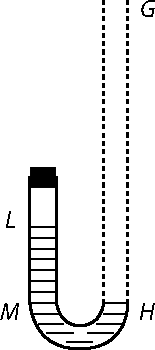
\includegraphics[width=0.15\textwidth]{gesamttex/edit_VIII-4/images/LH_37_04_149-150_d2_150r.pdf}
\edcaption[0.5em]{\lbrack \textit{Fig.\:2}\rbrack}
\end{edfigure}%
\newpage%
\pstart%
Fieri%
\edlabel{37_04_149-150_150r_03b}
etiam potest,
ob motum aeris vel alterius liquidi,%
\indexS{motus aeris}%
\indexS{motus liquidi}%
\indexS{aer motus}%
\indexS{liquidum motum}
ut
quae in eo natant%
\indexS{particulae natantes in aere}%
\indexS{particulae natantes in liquido}
non decidant%
\lbrack,\rbrack\
dum
\edtext{%
scilicet%
}{%
\lemma{scilicet}%
\Bfootnote{%
\textit{erg.\;L}%
}}
ipso motu rursus elevantur,%
\indexS{particulae elevatae motu aeris}%
\indexS{particulae elevatae motu liquidi}
atque ita alternis
nunc ascendentia,
nunc descendentia,
\edtext{%
revera%
}{%
\lemma{revera}%
\Bfootnote{%
\textit{erg.\;L}%
}}
manent in sublimi%
\indexS{particulae manentes in sublimi}
\edtext{%
donec
impetus ab externo impressus%
\indexS{impetus impressus ab externo}
elanguescat.%
}{%
\lemma{donec}%
\Bfootnote{%
impetus \lbrack...\rbrack\ impressus elanguescat
\textit{erg.\;L}%
}}
Quanquam haec minus ad institutum%
\indexS{institutum}
nostrum faciant,
quoniam quae motu%
\indexS{particulae elevatae motus aeris}%
\lbrack,\rbrack\
id est impresso%
\indexS{impetus impressus ab externo}%
\indexS{particulae elevatae impetu impresso}
\edtext{%
impetu%
\lbrack,\rbrack\
elevantur,%
\indexS{elevatio particularum impetu impresso}%
\indexS{impetus elevans particulas}
non sustinentur a liquore,%
\indexS{sustentatio particularum a liquore}%
\indexS{liquor sustinens particulas}%
}{%
\lemma{impetu}%
\Bfootnote{%
\textit{(1)}~sustentantur, %
\textit{(a)}~\textlangle--\textrangle\ %
\textit{(b)}~ipsi aeri %
\textit{(c)}~n\textlangle-- --\textrangle\ %
\textit{(2)}~elevantur, %
\textit{(a)}~vel %
\textit{(b)}~non sustinentur a liquore,%
~\textit{L}%
}}
atque adeo ad aequilibrium%
\indexS{aequilibrium particularum in liquore}
non conferunt.
\edtext{%
Nempe
(ut ex projectorum exemplo constat)%
\indexS{exemplum}
composito motu%
\indexS{motus compositus e gravitate et impetu}
feruntur ex gravitate%
\indexS{gravitas ferens particulas}
et impetu impresso.%
\indexS{impetus impressus ab externo}%
\indexS{impetus ferens  particulas}%
\indexS{latio particularum a gravitate et impetu}
Itaque gravitate%
\indexS{gravitas}
quidem continue cadunt,
sed cum concepto impetu%
\indexS{impetus conceptus}
magis vel saltem non minus eleventur,%
\indexS{impetus elevans particulas}
fit ut assurgant omnino
vel sustententur,%
\indexS{sustentatio particularum ab impetu}%
\indexS{impetus sustinens particulas}
non tamen a flu\textlangle ido\textrangle\
in quo suspenduntur.%
\indexS{suspensio particularum in fluido}%
\indexS{sustentatio particularum a fluido}%
\indexS{fluidum sustinens particulas}%
}{%
\lemma{Nempe}%
\Bfootnote{%
\textit{(1)}~continue %
\textit{(a)}~cadunt %
\textit{(b)}~cadere possu %
\textit{(c)}~cadunt ut %
\textit{(2)}~etsi inter cadendum %
\textit{(3)}~ex nisu gravitatis, etsi %
\textit{(4)}~(ut ex projectorum exemplo %
\textit{(a)}~cadunt %
\textit{(b)}~constat) composito %
\lbrack...\rbrack\ quo suspenduntur.
\textit{erg.\;L}%
}}
\pend%
\pstart%
Quae etiam
\edtext{%
causa confert ad%
}{%
\lemma{causa}%
\Bfootnote{%
\textit{(1)}~est cur %
\textit{(2)}~confert ad%
~\textit{L}%
}}
aerem ventis validis%
\indexS{aer sublevatus vento}%
\indexS{ventus sublevans aerem}
\edtext{%
sublevandum;
unde tempesta\lbrack s\rbrack\ futura%
\indexS{tempestas praenuntiata barometro}
saepe barometro praenuntiari potest%
\indexS{barometrum praenuntians tempestam}%
\lbrack,\rbrack\
quanquam praeterea
ventis nunc in diversa tendentibus%
\indexS{venti tendentes in diversa}
deduci aerem atque attenuari,%
\indexS{aer attenuatus ventis contrariis}%
\indexS{aer deductus ventis contrariis}
nunc concurrentibus condensari,%
\indexS{aer condensatus ventis concurrentibus}%
\indexS{venti concurrentes}
passim etiam ad fluctuum instar%
\indexS{fluctus}
nunc deprimi in valles%
\indexS{aer depressus in valles}%
\indexS{vallis}
nunc in montes attolli%
\indexS{aer elevatus in montes}%
\indexS{mons}
consentaneum videatur.
Quibus de rebus%
}{%
\lemma{sublevandum;}%
\Bfootnote{%
\textit{(1)}~eaque ventis est %
\textit{(2)}~et %
\textit{(3)}~unde %
\bars{tempestatem \textit{ändert Hrsg.}} %
\textit{(a)}~futuram %
\textit{(b)}~futura %
\bars{saepe \textit{erg.}} barometro %
\textit{(aa)}~praenuntiandam %
\textit{(bb)}~praenuntiari potest quanquam %
\textit{(aaa)}~eadem %
\textit{(bbb)}~praeterea ventis %
\textit{(aaaa)}~(praesertim si plures ad easdem aut diversas partes tendant) alicubi valles %
\textit{(bbbb)}~\bars{nunc in diversa tendentibus \textit{erg.}} deduci aerem atque attenuari %
\textit{(aaaaa)}~alibi et comprimi, %
\textit{(bbbbb)}~nunc conflictantibus %
\textit{(ccccc)}~aut in valles deprimi, alibi vero %
\textit{(ddddd)}~\bars{nunc concurrentibus \textit{erg.}} condensari %
\textit{(aaaaa-a)}~et ad fluctuum instar in montes attolli. %
\textit{(bbbbb-b)}~passim etiam \lbrack...\rbrack\ attolli consentaneum videatur.%
\textit{(aaaaa-aa)}~Quam in rem %
\textit{(bbbbb-bb)}~Quibus de rebus%
~\textit{L}%
}}
etiam
\edtext{%
Edmundus Hallejus%
\indexN{\textls{Halley} (Hali, Hallé, Hale, Hales, Hallaeus), Edmond 1656\textendash1742}
vir clarus%
\indexS{vir clarus}
nonnulla egregria est commentatus.%
}{%
\lemma{Edmundus \lbrack...\rbrack\ commentatus}%
\Cfootnote{%
Siehe E.\;\textsc{Halley},
"A discourse of the rule of the decrease of the height of the mercury"
(\textit{PT}~XVI, Nr.\;181, 25.\;Mai 1686, S.\;104--116).%
\cite{01526}%
}}%
\pend%
\vspace{1.0em}%
\pstart%
\noindent%
\lbrack%
\textit{Nachfolgender Textabschnitt (bis zu \refpassage{LH_37_04_149-150_150r_einschub}{LH_37_04_149-150_150r_einschub} ) in L am Rand ergänzt:}%
\rbrack\
\pend%
\vspace{0.5em}%
\pstart%
\noindent%
\edtext{%
Videri quidem posset
particulas calore sustentatas%
\indexS{particulae sustentatae calore}%
\indexS{calor sustinens particulas}%
\indexS{sustentatio particularum calore}
etiam ad rem non facere,
non magis quam
quae motu sustentantur,%
\indexS{sustentatio particularum motu aeris}
quia
cum sint aere paris spatii leviores,%
\indexS{particulae leviores aere paris spatii}%
}{%
\lemma{Videri}%
\Bfootnote{%
\textit{(1)}~etiam poterit %
\textit{(2)}~quidem posset particulas %
\textit{(a)}~heterogeneas %
\textit{(b)}~\bars{calore \textit{erg.}} in aere %
\textit{(c)}~calore sustentatas %
\textit{(aa)}~adeo aere pari\textlangle s\textrangle\ spatii leviores, non %
\textit{(bb)}~etiam ad rem %
\lbrack...\rbrack\ paris spatii leviores,%
~\textit{L}%
}}
cylindrum aereum%
\indexS{cylinder aereus}
potius leviorem reddant,
quam graviorem.
Sed respondendum est,
eo ipso
dum aer%
\indexS{aer recipiens materiam gravem}
novam materiam gravem%
\indexS{materia gravis recepta in aerem}
recipit,
fieri graviorem,%
\indexS{aer factus gravior}
\ledpb%
ut
cum lignum aquae innatat%
\indexS{lignum innatans aquae}%
\lbrack,\rbrack\
vas aquam continens%
\indexS{vas continens aquam}
gravius erit,
quam si lignum auferatur.
Itaque
\edtext{%
quod levior reddatur columna aeris%
\indexS{columna aeris}%
\indexS{aer redditus levior}%
\indexS{aer recipiens materiam leviorem}
ob materiam leviorem receptam%
\indexS{materia levior recepta in aerem}%
}{%
\lemma{quod}%
\Bfootnote{%
\textit{(1)}~leviorem %
\textit{(2)}~levior reddatur %
\textit{(a)}~cylinder %
\textit{(b)}~columnam %
\textit{(c)}~columna aeris %
\textit{(aa)}~materia leviore recepta %
\textit{(bb)}~ob materiam leviorem receptam%
~\textit{L}%
}}
intelligendum
\edtext{%
est de columna%
\indexS{columna aeris}
altitudinis ejusdem.%
\indexS{altitudo columnae aeris}%
}{%
\lemma{est}%
\Bfootnote{%
\textit{(1)}~de cylindro spatii pristini, cum %
\textit{(2)}~de columna altitudinis ejusdem.%
~\textit{L}%
}}
Hic vero consentaneum
\edtext{%
est
columnam%
\indexS{columna aeris}
reddi altiorem%
}{%
\lemma{est}%
\Bfootnote{%
\textit{(1)}~cylindrum reddi altius %
\textit{(2)}~columnam reddi altiorem%
~\textit{L}%
}}
materia nova recepta%
\indexS{materia nova recepta in aerem}
ac sustentata.%
\edlabel{LH_37_04_149-150_150r_einschub}%
\pend%
\vspace{1.0em}%
\pstart%
\noindent%
Explicata jam
\edtext{%
sustentatione%
\indexS{sustentatio particularum in aere}%
\lbrack,\rbrack\
ad aquam rursus delabentem%
\indexS{aqua delabens in aere}%
}{%
\lemma{sustentatione}%
\Bfootnote{%
\textit{(1)}~ad casum %
\textit{(2)}~ad aquam rursus delabentem%
~\textit{L}%
}}
veniamus.
\edtext{%
Itaque cum calore
factum sit
ut humores%
\indexS{humor inflatus in bullas}
velut in bullas quasdam%
\indexS{bulla inflata humore}
et ut ita dicam vesicas%
\indexS{vesica inflata humore}
inflarentur,
quae excluso%
}{%
\lemma{Itaque}%
\Bfootnote{%
\textit{(1)}~vel deferente calore,\indexS{calor deferens} %
\textit{(2)}~quemadmodum %
\textit{(3)}~cum calore factum sit ut humores %
\textit{(a)}~inflati in %
\textit{(b)}~velut in %
\lbrack...\rbrack\ vesicas inflarentur, %
\textit{(aa)}~quibus exclu %
\textit{(bb)}~ex quibus exclus %
\textit{(cc)}~quae excluso%
~\textit{L}%
}}
aere crassiore%
\indexS{aer crassior}%
\indexS{aer exclusus}
intus
\edtext{%
vacuae%
\indexS{bulla vacua intus}
ascenderant ad certam usque altitudinem%
\indexS{bulla ascendens}%
\indexS{ascensus bullae}
ibique sustentabantur,%
\indexS{bulla sustentata}%
\indexS{sustentatio bullae}%
}{%
\lemma{vacua}%
\Bfootnote{%
\textit{(1)}~velu %
\textit{(2)}~vel ascenderant vel sustentabantur, %
\textit{(3)}~ascenderant %
\bars{ad certam usque altitudinem ibique \textit{erg.}} sustentabantur,%
~\textit{L}%
}}
nunc
\edtext{%
vicissim eveniet ut%
}{%
\lemma{vicissim}%
\Bfootnote{%
eveniet ut
\textit{erg.\;L}%
}}
cessante calore%
\indexS{calor cessans}
instar vesicae flaccidae%
\indexS{vesica flaccida}
concidant,%
\indexS{bulla concidens}
et recuperata gravitate%
\indexS{gravitas recuperata}
delabentur.%
\indexS{bulla delabens}
Sed et aliae
\lbrack%
\href{\Scan{LH_37_04_150v}}	%
{150\,v\textsuperscript{o}}%
\rbrack\	
humorum%
\indexS{humor particulatus}
particulae,%
\indexS{particulae humoris}
non quidem clausae
sed
\edtext{%
potius%
}{%
\lemma{potius}%
\Bfootnote{%
\textit{erg.\;L}%
}}
ab aere ubique penetratae%
\indexS{aer penetrans particulam}%
\lbrack,\rbrack\
ob nimiam tamen tenuitatem,%
\indexS{tenuitas superficiei particulae}
id est superficiei%
\indexS{superficies particulae humoris}
magnitudinem,%
\indexS{magnitudo superficiei particulae}
perrumpere ac descendere non valentes%
\lbrack,\rbrack\
poterunt rursus addensari%
\indexS{particulae addensatae}
vel incrassari,%
\indexS{particulae incrassatae}
dum plures laminae tenuissimae conjunguntur inter se,%
\indexS{laminae tenues conjunctae}
sive ipso motu aeris%
\indexS{motus aeris}
dum sibi occurrentes implicantur
ac cohaerescunt%
\lbrack,\rbrack\
sive eo modo
quo videmus sales in aquis solutos%
\indexS{sal solutus in aqua}%
\indexS{solutio salis in aqua}
\edtext{%
paulatimque%
}{%
\lemma{paulatimque}%
\Bfootnote{%
\textit{erg.\;L}%
}}
in crystallos%
\indexS{crystallus}
reconcrescere;%
\indexS{sal reconcretus in crystallos}
sive denique
\edtext{%
superiorum partium jam
ex caloris vel motus cessatione%
\indexS{cessatio motus}%
\indexS{cessatio caloris}%
\indexS{motus cessans}%
\indexS{calor cessans}
descendentium lapsu;%
\indexS{lapsus particularum in aere}%
}{%
\lemma{superiorum}%
\Bfootnote{%
\textit{(1)}~lapsu %
\textit{(2)}~quae %
\textit{(3)}~partium jam %
\textit{(a)}~descenden %
\textit{(b)}~ex caloris %
\textit{(aa)}~defectu %
\textit{(bb)}~cessatione %
\textit{(cc)}~vel motus %
\textit{(aaa)}~descendentium, %
\textit{(bbb)}~cessatione descendentium lapsu;%
~\textit{L}%
}}
ita enim labentes guttae%
\indexS{gutta labens}
ut
\edtext{%
pilae%
\indexS{pila nivis}%
\indexS{nix}
ex nive%
}{%
\lemma{pilae}%
\Bfootnote{%
\textit{(1)}~nivis %
\textit{(2)}~ex nive%
~\textit{L}%
}}
inter eundum crescent.%
\indexS{gutta crescens inter eundum}
\pend%
\pstart%
Et fieri omnino potest,
ut nulla sit
\edtext{%
prorsus quorundam vaporum sustentatio,%
\indexS{sustentatio vaporis}%
\indexS{vapor sustentatus}
sed continue vel ascendant,%
\indexS{vapor ascendens}
vel descendant;%
\indexS{vapor descendens}
dissipentur%
\indexS{vapor dissipatus}%
\indexS{dissipatio vaporis}
autem ascensu%
\indexS{ascensus vaporis}%
}{%
\lemma{prorsus}%
\Bfootnote{%
\textit{(1)}~(nisi calore quorundam %
\textit{(2)}~, nisi a calore %
\textit{(3)}~sustentatio motu quorundam %
\textit{(4)}~quorundam %
\textit{(a)}~particularum %
\textit{(b)}~vaporum %
\textit{(aa)}~suscitatio %
\textit{(bb)}~sustentatio, sed continue %
\textit{(aaa)}~descendant %
\textit{(bbb)}~vel ascendant, vel descendant;
\textit{(aaaa)}~tractantur %
\textit{(bbbb)}~di %
\textit{(cccc)}~dissipentur autem ascensu%
~\textit{L}%
}}
(dum tenuissimae partes reliquas post se relinquant)
et rursus descensu%
\indexS{descensus vaporis}
recolligantur.%
\indexS{vapor recollectus in guttas}%
\indexS{recollectio vaporis in guttas}
Descendent autem lentissime%
\indexS{descensus vaporis}%
\indexS{vapor descendens}
dum
\edtext{%
tenu\lbrack es\rbrack%
}{%
\lemma{tenuia}%
\Bfootnote{%
\textit{L\;ändert Hrsg.}%
}}
sunt,
ob aeris resistentiam%
\indexS{resistentia aeris}%
\lbrack;\rbrack\
aucta autem mole %
imminutaque simul superficie,
tandem recolligentur in guttas,%
\indexS{vapor recollectus in guttas}%
\indexS{recollectio vaporis in guttas}
et cum impetu
\edlabel{37_04_149-150_150v_duza-1}%
delabentur.%
\indexS{vapor delabens}%
\indexS{delapsus vaporis}%
\edtext{}{%
\xxref{37_04_149-150_150v_duza-1}{37_04_149-150_150v_duza-2}%
\lemma{delabentur,}%
\Bfootnote{%
\textit{(1)}~Haec p %
\textit{(2)}~Ex %
\textit{(3)}~Atque ex his prinicpiis %
\textit{(a)}~putem %
\textit{(b)}~attente consideratis, et circumspecte adhibitis, putem %
\textit{(5)}~At %
\bars{%
\textit{(1)}~Quod %
\textit{(2)}~Quae igitur %
\textit{(a)}~sint %
\textit{(b)}~hujus %
\textit{(aa)}~sunt %
\textit{(bb)}~naturae sunt exhalationes %
\textit{(aaa)}~ipsae per se %
\textit{(aaaa)}~a b %
\textit{(bbbb)}~in barometro nihil mutabunt %
\textit{(bbb)}~ut nunquam %
\lbrack...\rbrack\ per se mutabunt, %
\textit{(aaaa)}~sed %
\textit{(bbbb)}~nisi dum %
\lbrack...\rbrack\ colligendo densadoque %
\textit{(aaaaa)}~sed satis ad descen %
\textit{(bbbbb)}~ad descendendum validas reddent. %
\textit{erg.}} %
\textit{(6)}~Atque ex \lbrack...\rbrack\ phaenomena putem%
~\textit{L}%
}}
Quae igitur hujus naturae%
\indexS{natura}
sunt exhalationes%
\indexS{exhalatio sustentata in aere}
ut nunquam sustententur in aere%
\lbrack,\rbrack\
in barometro%
\indexS{barometrum}
nihil per se mutabunt,
nisi dum alias in aere sustentatas%
\indexS{exhalatio sustentata in aere}
colligendo densandoque
ad descendendum validas reddent.
\pend%
\pstart%
Atque ex his principiis attente consideratis%
\indexS{principium consideratum}
et circumspecte adhibitis%
\indexS{principium adhibitum}
pleraque phaenomena%
\indexS{phaenomenon solutum e principiis}
putem%
\edlabel{37_04_149-150_150v_duza-2}
solvi posse,
praesertim
\edtext{%
si \lbrack accedant\rbrack\
\edtext{%
\edlabel{LH_37_04_149-150_150v_hllnwtn-1}%
quae viri ingeniosissimi%
\indexS{vir ingeniosus}
nuper de ventis regnantibus%
\indexS{ventus regnans}
et marium motu%
\indexS{motus maris}
sunt meditati.%
\edlabel{LH_37_04_149-150_150v_hllnwtn-2}%
}{%
\lemma{quae \lbrack...\rbrack\ meditati}%
\Cfootnote{%
Möglicherweise Anspielung auf
\textsc{E.\;Halley}, "The true theory of the tides, extracted from 'hat admired treatise of Mr.\;Isaac Newton intituled \textit{Philosophiae naturalis principia mathematica}"
(\textit{PT}~XIX, %
Nr.\;226, 31.\;März 1697, S.\;445--457).\cite{02593}\cite{00158}
Leibniz könnte aber auch auf folgenden Aufsatz anspielen:
\textsc{E.\;Halley}, "An historical account of the trade winds ... with an attempt to assign the physical cause" 
(\textit{PT}~XVI, %
Nr.\;183, 30.\;September 1686, S.\;153--168).\cite{02594}\cite{00158}%
\indexN{\textls{Halley} (Hali, Hallé, Hale, Hales, Hallaeus), Edmond 1656\textendash1742}%
\indexN{\textls{Newton} (Neutonus), Isaac 1643\textendash1727}%
}}
Horum autem omnium%
}{%
\lemma{si}%
\Bfootnote{%
\bars{accedant \textit{gestr., wieder gültig macht Hrsg.}} quae
\textit{(1)}~clari %
\textit{(2)}~viri ingniossimi %
\textit{(a)}~\textlangle Astronomicis principiis\textrangle\ %
\textit{(b)}~nuper de ventis regnantibus %
\bars{et marium motu sunt \textit{erg.}} meditati
\textit{(aa)}~sunt, %
\textit{(bb)}~conjugentur. Nam quibus %
\textit{(2)}~. Horum autem %
\bars{omnium \textit{erg.}}\textit{L}%
}}
rationes
partim a sole%
\indexS{sol}
et luna,%
\indexS{luna}
partim a motu%
\indexS{motus terrae}
\edtext{%
terrae,%
\indexS{terra}
partim a diversa partium telluris%
\indexS{partes telluris}%
\indexS{tellus}
conditione%
\indexS{conditio partium telluris}
desumendas%
}{%
\lemma{terrae}%
\Bfootnote{%
\bars{partim a diversa partium %
\textit{(1)}~terrae conditione \textlangle--\textrangle\ %
\textit{(2)}~telluris conditione \textit{erg.}} %
\textit{(1)}~provenire %
\textit{(2)}~desumendas%
~\textit{L}%
}}
multa ostendunt phaenomena.%
\indexS{phaenomenon ostendens rationes}
Nec dubito
si majore in his attentione%
\indexS{attentio hominum}
versarentur homines%
\indexS{homo} %
conferrentque operas%
\indexS{operae hominum collatae} %
et ab iis excitarentur %
ad quos reipublicae cura%
\indexS{cura reipublicae}%
\indexS{respublica}
pertinet,
multa quae fiunt explicari,%
\indexS{facta explicata}
et quae futura sunt
\edtext{%
praevideri %
\indexS{futura praevista}
caverique%
}{%
\lemma{praevideri,}%
\Bfootnote{%
\textit{(1)}~caverique %
\textit{(2)}~posse, %
\textit{(3)}~magn %
\textit{(4)}~caverique%
~\textit{L}%
}}
si mala sunt,
aut si bona %
obtineri posse,
quae
\edtext{%
nunc casui%
\indexS{casus}%
}{%
\lemma{nunc}%
\Bfootnote{%
\textit{(1)}~fortunae\indexS{fortuna} %
\textit{(2)}~casui%
~\textit{L}%
}}
committuntur.
\pend%
\vspace{1.0em}%
\pstart%
\noindent%
\lbrack\textit{Der nachfolgende, abschließende Textabschnitt könnte womöglich nachträglich in~L ergänzt worden sein:}\rbrack%
\pend%
\newpage%
\pstart%
\noindent%
\edlabel{LH_37_04_149-150_150v_Camerarius-1}%
\edtext{%
(Itaque magnam laudem%
\indexS{laus magna}
merentur egregii viri%
\indexS{vir egregius}
Reiselius%
\indexN{\textls{Reisel} (Reyselius, Risselius, Reuschius), Salomon 1625\textendash1702}
et Camerarius%
\indexN{\textls{Camerarius}, Rudolf Jakob 1665\textendash1721}
quod et
\edtext{%
ipsi faciunt observationes%
\indexS{observatio de motu maris}
et alios ad easdem faciendas excitant.%
\edlabel{LH_37_04_149-150_150v_Camerarius-2}%
\lbrack)\rbrack%
}{%
\lemma{(Itaque}%
\Bfootnote{%
magnam \lbrack...\rbrack\ faciendas excitant.%
~\textit{erg.\;L}%
}}%
}{%
\lemma{ipsi \bracks{...} excitant}%
\Cfootnote{%
Siehe
\textsc{R.\:J.\;Camerarius}, \textit{Ephemerides meteorologicae} (Augsburg 1696);\cite{01445}
dort erklärt die Praefatio (S.\;5\,f.), mit welchen Absichten Wetterbeobachtungen in den Jahren 1691 bis 1694 durchgeführt und in der Abhandlung (S.\;36--105) veröffentlicht worden seien.
Sowohl Camerarius (a.a.O., Descriptio instrumenti, S.\;11)\cite{01445} wie auch Ramazzini\indexN{\textls{Ramazzini} (Ramazzinus), Bernardino 1633\textendash1714} (\textit{Ephemerides barometricae}, 1695, S.\;7\,f.;\cite{01516} 1696, S.\;3)\cite{01517} verweisen ferner auf \textsc{S.\;Reisel}, "Cogitatio de thermometro correspondente" (\textit{AL1}, decuria~III, annus~I, 1694, Appendix, S.\;1--12),\cite{02592} wo ein Instrument geschildert wird, das eine kollektive systematische Erhebung thermometrischer Daten ermöglichen soll.
Reisel erwähnt dort (S.\;5) auch eigene Wetterbeobachtungen.%
}}
\pend%
\pstart%
Sequentes interim propositiones notari velim,%
\indexS{propositio}
quarum pars
\edtext{%
etiam in
\edtext{%
nostr\lbrack o\rbrack\ olim edito libello physico%
\indexS{libellum physicum}%
}{%
\lemma{nostro \lbrack...\rbrack\ physico}%
\Cfootnote{%
Siehe G.\:W.\;\textsc{Leibniz},
\textit{Hypothesis physica nova}
(Mainz 1671;
\textit{LSB} VI,\;2 N.\;40).%
\cite{00256}%
}}%
}{%
\lemma{etiam}%
\Bfootnote{%
\textit{(1)}~ex %
\textit{(2)}~in \bars{nostra \textit{ändert Hrsg.}} olim %
\textit{(a)}~edita Hypo %
\textit{(b)}~edito libello physico%
~\textit{L}%
}}
tradita
\edlabel{37_04_149-150_150v_09a}%
est%
\lbrack:\rbrack%
\edtext{}{%
\xxref{37_04_149-150_150v_09a}{37_04_149-150_150v_10b}%
\lemma{est}%
\Bfootnote{%
\lbrack/\rbrack\
\textit{(1)}~(1)~Quod in liquido\indexS{liquidum} cadit, %
\textit{(a)}~cum ipso non gravitationem suam %
\textit{(b)}~non exercet %
\textit{(2)}~(1) %
\textit{(a)}~Liquores\indexS{liquor} %
\textit{(b)}~Vapores in aere per calorem ascendentes\indexS{vapor ascendens in aere per calorem} %
\textit{(c)}~Quae calore in bullas intus %
\textit{(aa)}~vacuas %
\textit{(bb)}~inflantur %
\textit{(cc)}~aere %
\textit{(dd)}~vacuas inflata \lbrack...\rbrack\ destillationum chemicarum. %
\lbrack/\rbrack\ 
\textit{(aaa)}~(2)~Quae per motum in liquido elevantur et concepto impetu sustinentur in liqui %
\textit{(bbb)}~(2)~\bars{Gravia~\textit{erg.}} quae motu %
\textit{(aaaa)}~in liquido eleva %
\textit{(bbbb)}~fluido %
\textit{(cccc)}~elevanur et concepto impetu sustinentur %
\textit{(aaaaa)}~in liquido %
\textit{(bbbbb)}~in fluido, %
\lbrack...\rbrack\ non sustentantur %
\textit{(aaaaa-a)}~nec cum ipso gravitationem suam exercent, sed %
\textit{(aaaaa-aa)}~cadunt etiam %
\textit{(bbbbb-bb)}~cadunt etiamsi non proficiant cadendo %
\textit{(bbbbb-b)}~. %
\bars{Hinc patet \lbrack...\rbrack\ vehementer aguntur. \textit{erg.}} %
\lbrack/\rbrack\ (3) Quod in %
\textit{(aaaaa-aa)}~liquore cada %
\textit{(bbbbb-bb)}~fluido %
\textit{(aaaaa-aaa)}~\bars{grave \textit{streicht Hrsg.}} %
\textit{(bbbbb-bbb)}~cadit grave, %
\lbrack...\rbrack\ non exercet, %
\bars{neque \textit{ändert Hrsg.}} fundum vel oppositum onus premit.%
~\textit{L}%
}}%
\pend%
\pstart%
\noindent%
(1)
Quae calore%
\indexS{calor}
in bullas intus vacuas%
\indexS{bulla vacua intus}
inflata in aere assurgunt,
refrigerata
instar vesicae flaccescentis%
\indexS{vesica flaccescens}
gravitatem recipiunt.%
\indexS{gravitas recepta}
Haec illustrant naturam%
\indexS{natura destillationis chemicae}
destillationum%
\indexS{destillatio chemica}
chemicarum.%
\pend%
\pstart%
\noindent%
(2)
Gravia quae motu elevantur%
\indexS{grave elevatum motu}%
\indexS{motus elevans grave}
et concepto impetu sustinentur%
\indexS{grave sustentum impetu concepto}%
\indexS{impetus conceptus}
in fluido,%
\indexS{grave sustentum in fluido}
ab ipso fluido non sustentantur.
Hinc patet
gravitatem aeris%
\indexS{gravitas aeris minuta ventis}
ventis minui posse%
\indexS{ventus minuens gravitatem aeris}
cum nubes ab ipsis vehementer aguntur.%
\indexS{nubes actae a ventis}
\pend%
\pstart%
\noindent%
(3)
Quod in fluido %
cadit grave,%
\indexS{grave cadens in fluido}%
\indexS{fluidum grave}
cum ipso gravitationem suam non exercet,%
\indexS{gravitatio gravis}%
\indexS{gravitatio exercita}
\lbrack donec\rbrack\
fundum vel oppositum onus%
\indexS{fundus}%
\indexS{onus oppositum}
premit.%
\edlabel{37_04_149-150_150v_10b}
\edtext{%
Hinc pluvius aer sereno levior,%
\indexS{aer pluvius}%
\indexS{aer serenus}%
\indexS{aer levior}
minusque sustinet Hydrargyrum in Barometro.%
\indexS{aer sustinens hydrargyrum}%
\indexS{hydrargyrum in barometro}%
\indexS{barometrum}%
}{%
\lemma{Hinc}%
\Bfootnote{%
pluvius aer %
\textit{(1)}~gravior %
\textit{(2)}~sereno levior, %
\lbrack...\rbrack\ in Barometro.
\textit{erg.\;L}%
}}%
\pend%
\pstart%
\noindent%
(4)
\edtext{%
Omne fluidum%
\indexS{fluidum}
habet gradum%
}{%
\lemma{omne}%
\Bfootnote{%
\textit{(1)}~liquidum %
\textit{(2)}~quod gradum %
\textit{(3)}~fluidum habet gradum%
~\textit{L}%
}}
aliquem tenacitatis.%
\indexS{gradus tenacitatis fluidi}%
\indexS{tenacitas fluidi}
\edtext{%
Hujus usus contra atomos%
\indexS{atomi}
et materiam%
\indexS{materia subtilis primi elementi}
\edtext{%
quam vocant subtilem primi elementi.%
\indexS{elementum primum}%
}{%
\lemma{quam \lbrack...\rbrack\ elementi}%
\Cfootnote{%
Anspielung auf die kartesische Elementenlehre;%
\indexN{\textls{Descartes} (Cartesius, des Cartes), René 1596\textendash1650}
s‚†iehe etwa R.\;\textsc{Descartes},
\textit{Le monde}, cap.\;V
(Paris 1664, S. 49--51;\cite{02532}
\textit{DO} XI, S.\;24.3--28).\cite{00120}%
}}
}{%
\lemma{Hujus}%
\Bfootnote{%
usus \lbrack...\rbrack\ primi elementi.
\textit{erg.\;L}%
}}
\pend%
\newpage%
\pstart%
\noindent%
\edtext{%
(5)
Fluidum tenacitate sua resistit%
\indexS{fluidum resistens proportione superficiei}%
\indexS{tenacitas fluidi}
proportione superficiei perrumpentis.%
\indexS{superficies perrumpentis}
Hinc%
}{%
\lemma{(5)}%
\Bfootnote{%
\textit{(1)}~Tenacis %
\textit{(2)}~Fluidum tenacitate sua resistit %
\textit{(a)}~perrumpenti, %
\textit{(b)}~proportione superficiei perrumpentis. %
\textit{(aa)}~Quae %
\textit{(bb)}~Hinc%
~\textit{L}%
}}
fit ut divisa in partes exiguas,%
\indexS{divisum in partes exiguas}%
\indexS{pars exigua}
minus toto continuo possint.%
\indexS{totum continuum}
\pend%
\pstart%
\noindent%
(6)
Grave in fluido suspendi potest,%
\indexS{grave suspensum in fluido}%
\indexS{suspensio gravis in fluido}
\edtext{%
si tam magna sit superficies%
\indexS{proportio superficiei corporis}
proportione exigui corporis,%
\indexS{corpus exiguum}
ut major sit resistentia a fluidi tenacitate,%
\indexS{resistentia a tenacitate fluidi}%
\indexS{tenacitas fluidi}
quam nisus a corporis gravitate.%
\indexS{nisus a gravitate corporis}%
\indexS{gravitas corporis}%
}{%
\lemma{si}%
\Bfootnote{%
\textit{(1)}~minor sit vis %
\textit{(2)}~tam magna %
\lbrack...\rbrack\ a corporis gravitate.%
~\textit{L}%
}}
\pend%
\pstart%
\noindent%
(7)
Iisdem positis
ex sola corporum complicatione%
\indexS{complicatio corporum}
descensus fieri potest.%
\indexS{descensus e complicatione corporum}
Hinc
\edtext{%
crystallismi salium illustrantur.%
\indexS{crystallismus salis}%
}{%
\lemma{crystallismi}%
\Bfootnote{%
\textit{(1)}~illustrantur %
\textit{(2)}~salium illustrantur.%
~\textit{L}%
}}
\pend%
\pstart%
\noindent%
(8)
Motu terrae %
lucisque circa terram,%
\indexS{motus terrae}%
\indexS{motus lucis circa terram}%
\indexS{terra}%
\indexS{lux}
\edtext{%
et actione%
}{%
\lemma{et}%
\Bfootnote{%
\textit{(1)}~pressione\indexS{pressio lunae} %
\textit{(2)}~actione%
~\textit{L}%
}}
lunae%
\indexS{actio lunae}%
\indexS{luna}%
\lbrack,\rbrack\
motus certi in aere et aquis nascuntur,%
\indexS{motus in aere}%
\indexS{motus in aquis}
de quibus
\edtext{%
\edtext{%
Keplerus,%
\indexN{\textls{Kepler} (Keplerus), Johannes 1571\textendash1630}
Galilaeus,%
\indexN{\textls{Galilei} (Galilaeus, Galileus), Galileo 1564\textendash1642}
Cartesius,%
\indexN{\textls{Descartes} (Cartesius, des Cartes), René 1596\textendash1650}%
}{%
\lemma{Keplerus,}%
\Bfootnote{%
\textit{(1)}~Cartesius, %
\textit{(2)}~Galilaeus, Cartesius,%
~\textit{L}%
}}
Is.\;%
\edtext{%
Vossius,%
\indexN{\textls{Vossius}, Isaac 1618\textendash1689}
Newtonius,%
\indexN{\textls{Newton} (Neutonus), Isaac 1643\textendash1727}
Mariottus,%
\indexN{\textls{Mariotte}, Edme, Seigneur de Chazeuil ca. 1620\textendash1684}%
}{%
\lemma{Vossius,}%
\Bfootnote{%
\textit{(1)}~Ma\textlangle riottus\textrangle\ %
\textit{(2)}~Newtonius, Mariottus,%
~\textit{L}%
}}
Hallejus,%
\indexN{\textls{Haak} (Haackius, Haakius, Hack), Theodor 1605\textendash1690}%
}{%
\lemma{Keplerus \bracks{...} Hallejus}%
\Cfootnote{%
Sämtliche Verweise sind nicht ermittelt worden.%
}}
\edtext{%
nos olim in \textit{Hypothesi}.%
}{%
\lemma{nos olim in \textit{Hypothesi}}%
\Cfootnote{%
Vgl. \textsc{Leibniz}, \textit{Hypothesis physica nova} §\,13 (Mainz 1671; \textit{LSB} VI,\;2 N.\;40, S.\;226\,f.).\cite{00256}%
}}
\pend%
\pstart%
\noindent%
(9)
\edtext{%
Hi motus quominus ubique %
sint%
\lbrack,\rbrack%
}{%
\lemma{Hi}%
\Bfootnote{%
\bars{motus \textit{erg.}}
quominus
\textit{(1)}~statim %
\textit{(2)}~\bars{ubique \textit{erg.}}
\bars{stati \textit{streicht Hrsg.}} sint%
~\textit{L}%
}}
diversae partium superficiei telluris conditiones faciunt,%
\indexS{tellus}%
\indexS{superficies telluris}%
\indexS{partes superficiei telluris}
quanquam et hae cum sint durabiles%
\lbrack,\rbrack\
latere aliquam regularitatem oporteat%
\indexS{regularitas}
sub ipsa irregularitate apparente.%
\indexS{irregularitas apparens}%
\pend%
\selectlanguage{latin}%
\frenchspacing%
\normalsize%
